% Compile with XeLaTeX or LuaLaTeX
\documentclass[10pt,a4paper]{article}
\usepackage{xcolor}
\usepackage{titlesec}
\usepackage{fontspec}
\defaultfontfeatures{Mapping=tex-text}
\usepackage{xunicode}
\usepackage{xltxtra}
\usepackage{polyglossia}
\usepackage{indentfirst}             % 段首缩进

\setdefaultlanguage{english}
% 设置字体
\setsansfont{Calibri}
\setmainfont[BoldFont=SimHei]{STKaiti}
\usepackage{amsmath}
\usepackage{amsfonts}
\usepackage{amssymb}
\usepackage{graphicx}
% 设置页边距
%\usepackage[left=2cm,right=2cm,top=2cm,bottom=2cm]{geometry}
% MATLAB代码插入包
\usepackage{listings}
\usepackage[framed,numbered,autolinebreaks,useliterate]{mcode}
% 新定义字体
\newfontfamily\song{SimSun}          % 宋体
\newfontfamily\hei{SimHei}           % 黑体
\XeTeXlinebreaklocale "zh"           % 中文断行

% Define light and dark Microsoft blue colours
\definecolor{MSBlue}{rgb}{.204,.353,.541}
\definecolor{MSLightBlue}{rgb}{.31,.506,.741}
% Define a new fontfamily for the subsubsection font
% Don't use \fontspec directly to change the font
\newfontfamily\subsubsectionfont[Color=MSLightBlue]{Times New Roman}
% Set formats for each heading level
\titleformat*{\section}{\Large\bfseries\sffamily\color{MSBlue}}
\titleformat*{\subsection}{\large\bfseries\sffamily\color{MSLightBlue}\song}
\titleformat*{\subsubsection}{\itshape\subsubsectionfont}

\author{邸明轩\footnote{email: mingxuandi@163.com}\\[2ex]
\\[2ex]}
\title{牛熊市试验报告 \uppercase\expandafter{\romannumeral1}}
\date{08, 07, 2016}
\begin{document}

%%%% 段落首行缩进两个字 %%%%
\makeatletter
\let\@afterindentfalse\@afterindenttrue
\@afterindenttrue
\makeatother
\setlength{\parindent}{2em}  %中文缩进两个汉字位

\maketitle

\section{Result }
评测标准:\\
P=Precision,预测结果中正确的比率;R=Recall,正确结果中被正确预测的比率 \\
F1是P与R的单调函数,取值范围为[0,1],数值越大表明模型的性能越好,F1取1时模型预测完全正确
\begin{equation}
		\label{eq:u0}
\begin{aligned}
F1=\dfrac{2*P*R}{P+R} 
\end{aligned}
\end{equation}
总共统计了126个月。\\
振幅阈值设为3\%时,判定牛市:45,熊市:33,震荡:48\\
3\%的月度增幅,半年化后收益大约为19.4\%,年化后收益为42.6\%。\\
F1准确率: 0.6127 (0.0999)\\
具体结果见图\ref{fig0}
\begin{figure}[t]
	\centering
	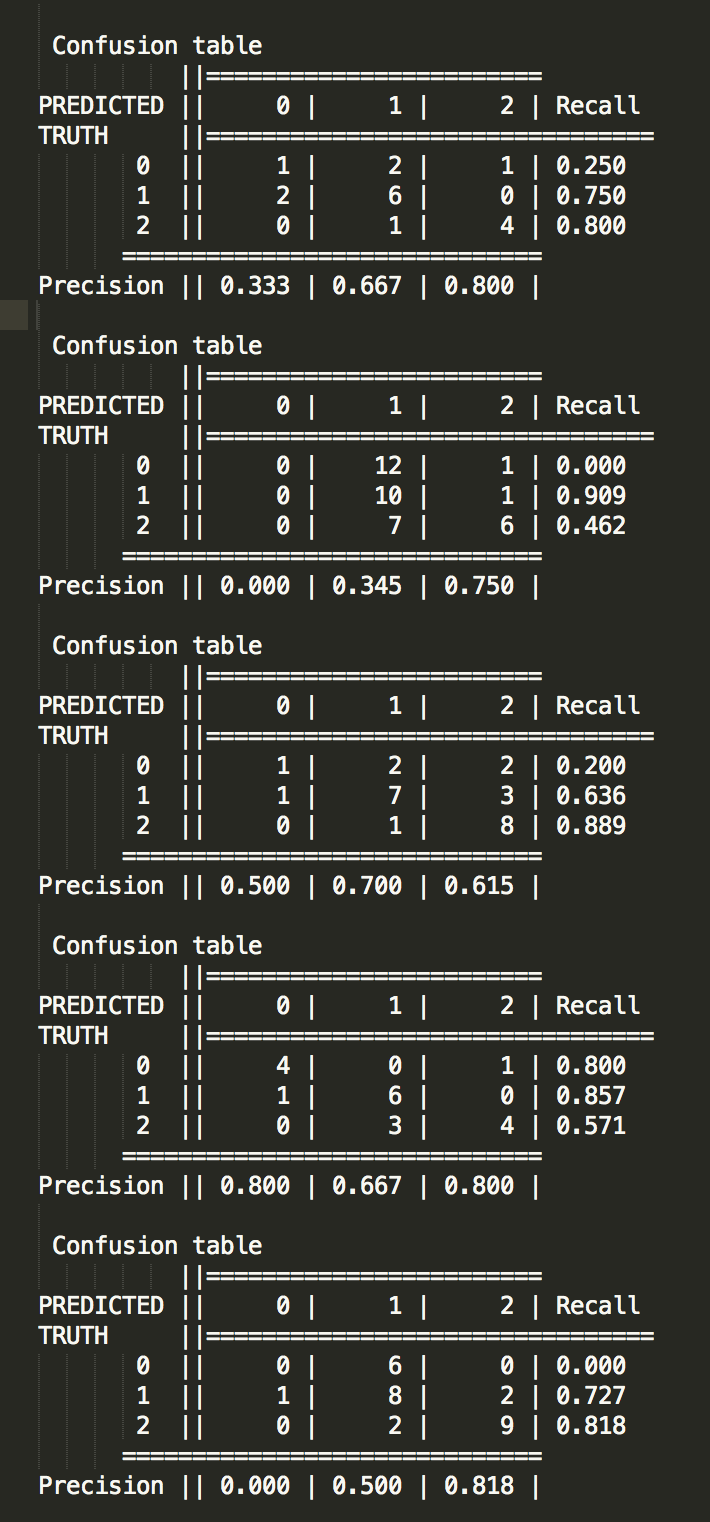
\includegraphics[width=0.9\linewidth]{result}
	\caption{预测的准确率记录。}
	\label{fig0}
\end{figure} 

\section{Next Step}

\begin{enumerate}
	\item 利用Scikit-Learn开发出可以单独运行的脚本程序。
	\item 在牛、熊市的样本中做采样,平衡训练数据,提高牛、熊市的预测准确率。
	\item 改进特征的表达方式,提高预测的准确率。
	\item 添加新的特征,包括当前时间新的信息提取的特征以及过去时间提取的特征。
\end{enumerate}
		
\section{Relation between feature and market}


\begin{figure}[t]
	\centering
	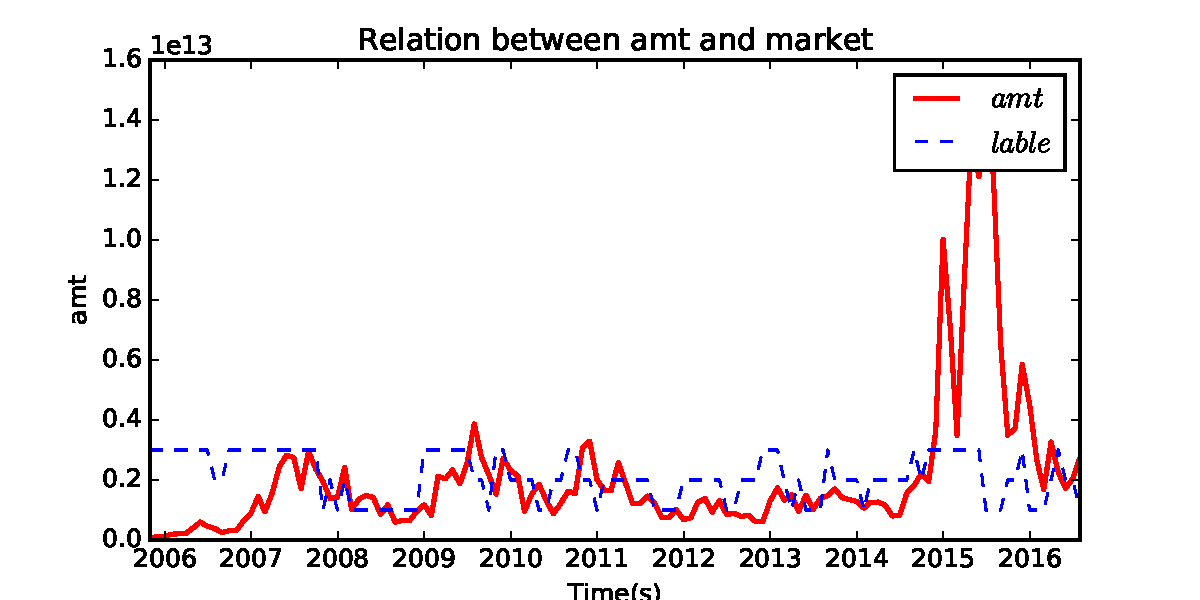
\includegraphics[width=0.9\linewidth]{amt.pdf}
	\caption{成交额(amt)与股市牛(高)、熊(低),震荡(中)的关系。}
	\label{fig1}
\end{figure}
\begin{figure}[t]
	\centering
	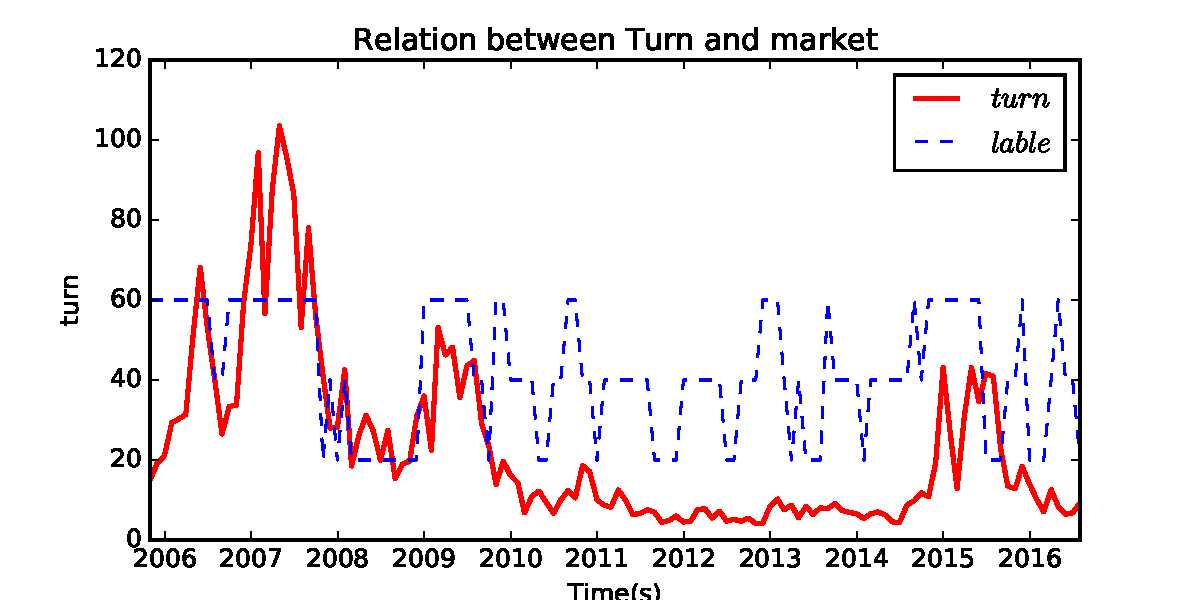
\includegraphics[width=0.9\linewidth]{turn.pdf}
	\caption{换手率(turn)与股市牛(高)、熊(低),震荡(中)的关系。}
	\label{fig2}
\end{figure}
\begin{figure}[t]
	\centering
	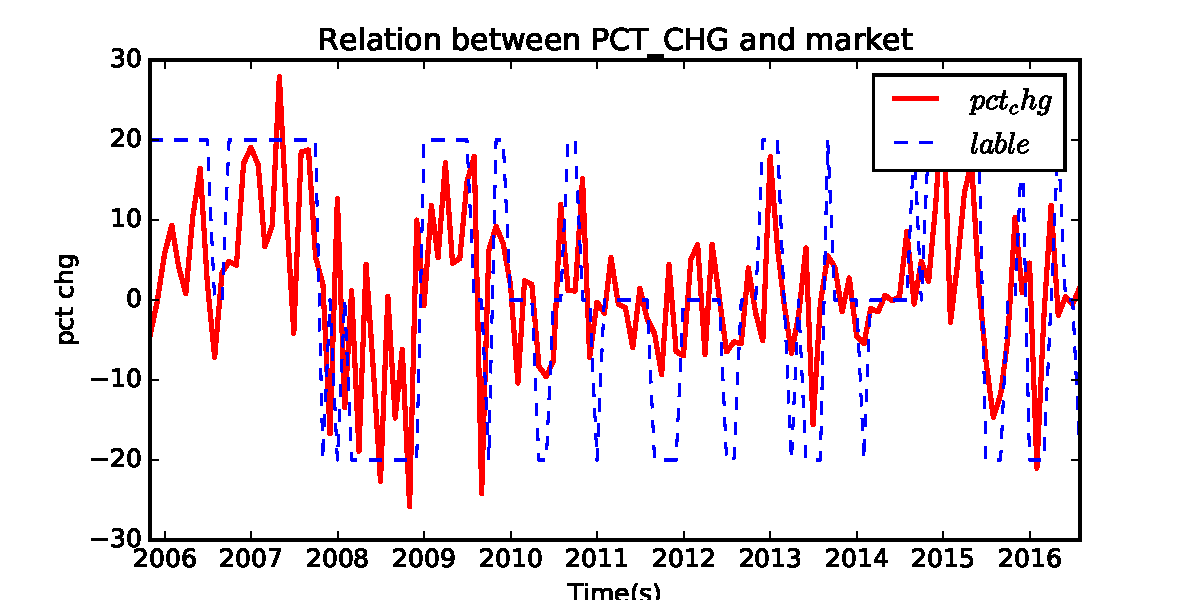
\includegraphics[width=0.9\linewidth]{PCT.pdf}
	\caption{涨跌幅($pct_chg$)与股市牛(高)、熊(低),震荡(中)的关系。}
	\label{fig3}
\end{figure}
\begin{figure}[t]
	\centering
	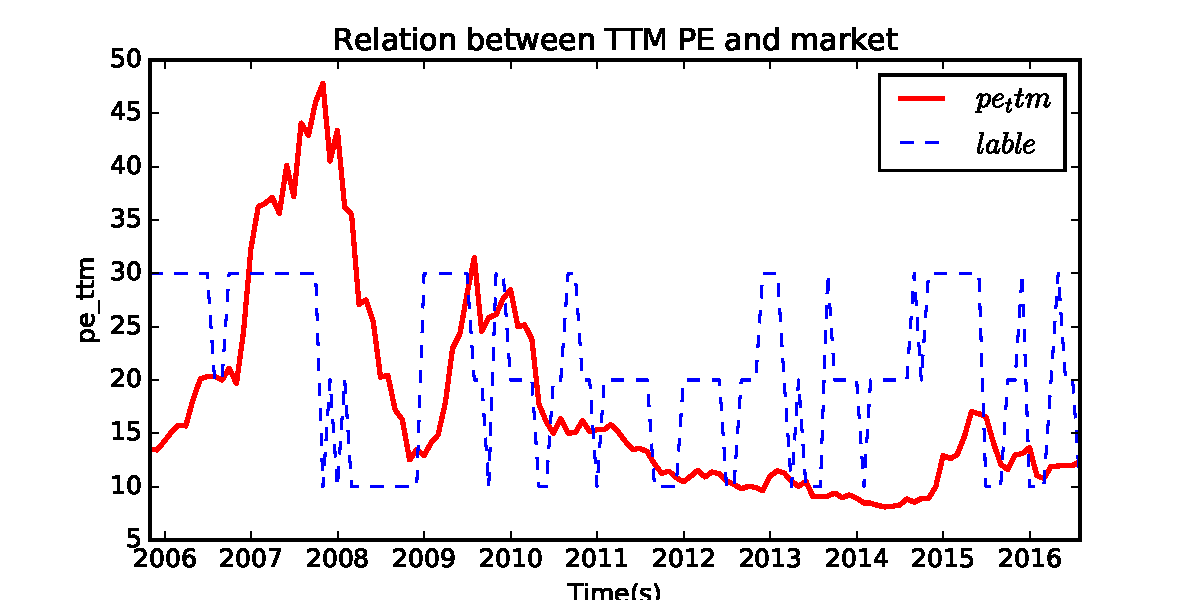
\includegraphics[width=0.9\linewidth]{PE.pdf}
	\caption{TTM PE与股市牛(高)、熊(低),震荡(中)的关系。}
	\label{fig4}
\end{figure}
\end{document}